\documentclass[12pt]{report}

% Essential packages
% \usepackage[french]{babel}
% \usepackage[T1]{fontenc}

\usepackage[margin=2cm]{geometry} % decrease margin
\usepackage{graphicx} % include images
\usepackage{hyperref} % urls, hyperlinks, etc
\usepackage{pdfpages} % include pdf pages
\usepackage{enumitem} % customize itemize
\usepackage[backend=bibtex]{biblatex} % bibliography
\usepackage{csquotes} % Quote bibliography and add hyperlinks
\usepackage{titlesec} % Modify chapter headings
\usepackage{wrapfig} % wrap text around figures
\usepackage{float} % force figure positions at the end of the file
\usepackage[linesnumbered,ruled,vlined]{algorithm2e}

\addbibresource{biblio.bib}

% Customize itemize item markers
\renewcommand\labelitemi{-}

% Add source to figures caption
\newcommand*{\captionsource}[2]{%
    \caption[{#1}]{%
        #1%
        \\\hspace{\linewidth}%
	\textbf{Source:} \textit{#2}%
    }%
}

% Some settings for the title page
\titleformat{\chapter}[display]{\normalfont\huge\bfseries}{}{0pt}{\Huge}
\titlespacing*{\chapter} {0pt}{20pt}{40pt}

% Force footnotes to stay on one page
\interfootnotelinepenalty=10000

\begin{document}

\begin{titlepage}
    \newcommand{\HRule}{\rule{\linewidth}{0.5mm}} % Defines a new command for the horizontal lines, change thickness here

    \centering
    \begin{minipage}{.25\textwidth}
	    \centering
	    
\includegraphics[width=80pt]{imgs/ENSIMAG.png}\\[1cm]
    \end{minipage}%
    \begin{minipage}{.25\textwidth}
	    \centering
	    
\includegraphics[width=80pt]{imgs/uga-logo.png}\\[1cm]
    \end{minipage}%
    \begin{minipage}{.25\textwidth}
	    \centering
	    
\includegraphics[width=80pt]{imgs/ryax-logo.png}\\[1cm]
    \end{minipage}%
    \begin{minipage}{.25\textwidth}
	    \centering
	    \includegraphics[width=80pt]{imgs/logo-LIG.jpg}\\[1cm]
    \end{minipage}

    \vspace{4cm}
    \textsc{\Large End of Studies Master's Project}\\[0.5cm]
    \textsc{\large Master's Thesis}\\[0.5cm]

    \HRule \\[0.4cm]
    { \huge \bfseries Simulation of a Kubernetes Cluster with Validation in Real Conditions}\\[0.4cm]
    \HRule \\[3cm]

    \begin{minipage}{0.4\textwidth}
        \begin{flushleft}
            \large
	    \textit{Author}\\
            Théo \textsc{Larue}
        \end{flushleft}
    \end{minipage}
    ~
    \begin{minipage}{0.4\textwidth}
        \begin{flushright}
            \large
	    \textit{Evaluator}\\
	    Surname \textsc{NAME}
        \end{flushright}
    \end{minipage}

    \vspace{2cm}

    \vspace{2cm}
    \vfill
    \textsc{\large February 24th to August 7th 2020}\\[0.5cm]


\end{titlepage}

\tableofcontents
\newpage

\chapter{Introduction}


In the early stages of application development, organizations used to run their
services on physical servers. With this direct approach came a few
problematics: resources allocation, maintainability, scalability for exemple.
Developers then went on with virtualized machines to run their services
regardless of physical infrasctucture, which then led to the concept of
containers.

\begin{figure}[]
	\centering
	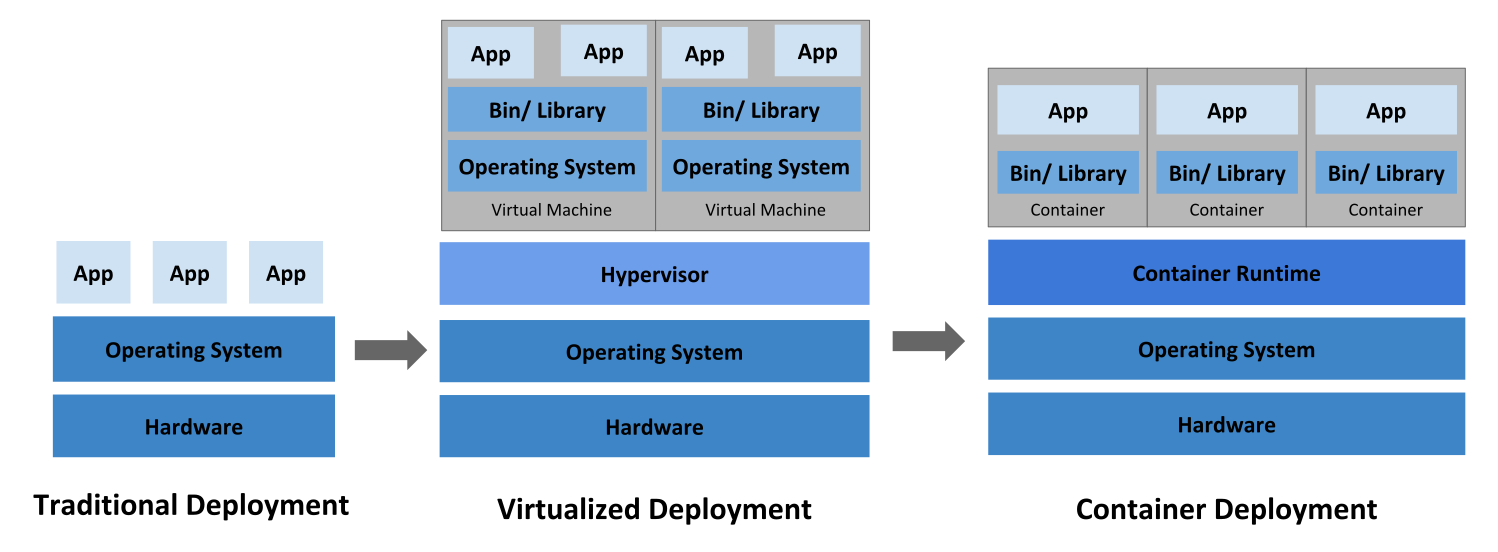
\includegraphics[width=\textwidth]{imgs/container_evolution.png}
	\captionsource{Evolution of application deployment.}{https://kubernetes.io/docs/concepts/overview/what-is-kubernetes/}
	\label{fig:container-evolution}
\end{figure}

Containers can be thought of as lightweight virtual machines.  Containerized
applications are applications running inside of a container, completely
independently of the underlying physical infrastructure. There are many
benefits to this : separating the development from deployment,
portability, easy resource allocation, breaking large services into smaller
micro-services or support of continuous integration tools, to cite a few.\\

Kubernetes\cite{kubernetes} allows the automation of the process of deploying, maintaining and
scaling containerized applications. It is an open source platform originally
designed by Google and now maintained and developed by the Cloud Native
Computing Foundation. It is industry grade and widely used by web services, big
or small, for its ease of use and its reliability.

However, eventhough it allows the automation of technical tasks that used to be
done manually, it doesn't take away other problematics like scheduling.
Scheduling is the NP-complete problem of allocating containers on physical
machines : one has to take into account resource availability, latency between
servers, storage locality, etc. Kubernetes schedulers have to handle this
difficult task of allocating resources in the most efficient way.

Thanks to the architecture of Kubernetes which is built around a central
component, the API server, schedulers can be developed independently in order
to fit particular needs. As a matter of fact, one universal scheduler that
would efficiently operate on any infrastructure will most likely never exist
and organizations often develop their own scheduler to better fit their needs.

This raises the question of scheduler development. Developing a scheduler
implies being able to test its performances throughout the development process,
however, testing in real conditions is time consuming and expensive.
Organizations can either have enough resources to cover these costs, or test
their scheduler against a simulation.\\

Kubernetes cluster simulations is an open problem and is the subject of this
master project. Our approach relies on the Batsim\cite{batsim} infrastructure
simulator, which is itself built upon Simgrid\cite{simgrid}. Batsim is
currently mostly used to simulate HPC infrastructures but was designed to be
able to simulate any kind of infrastructure and therefore is theoretically able
to simulate any Kubernetes cluster, moreover, Kubernetes was designed to run
services but is capable of handling High-Performance
Computing\cite{kube-for-hpc}. This project aims at adapting Batsim so it can
evaluate Kuberenetes schedulers.

\chapter{Problematic}

\section{Objectives}

The goal of this project is to design and implement Batkube, which will be an
interface between Batsim and Kubernetes schedulers. With this interface, we
want to compare Batsim results gainst data from a real Kubernetes cluster,
given HPC workloads.

\section{Kubernetes concepts}

\begin{figure}[]
	\centering
	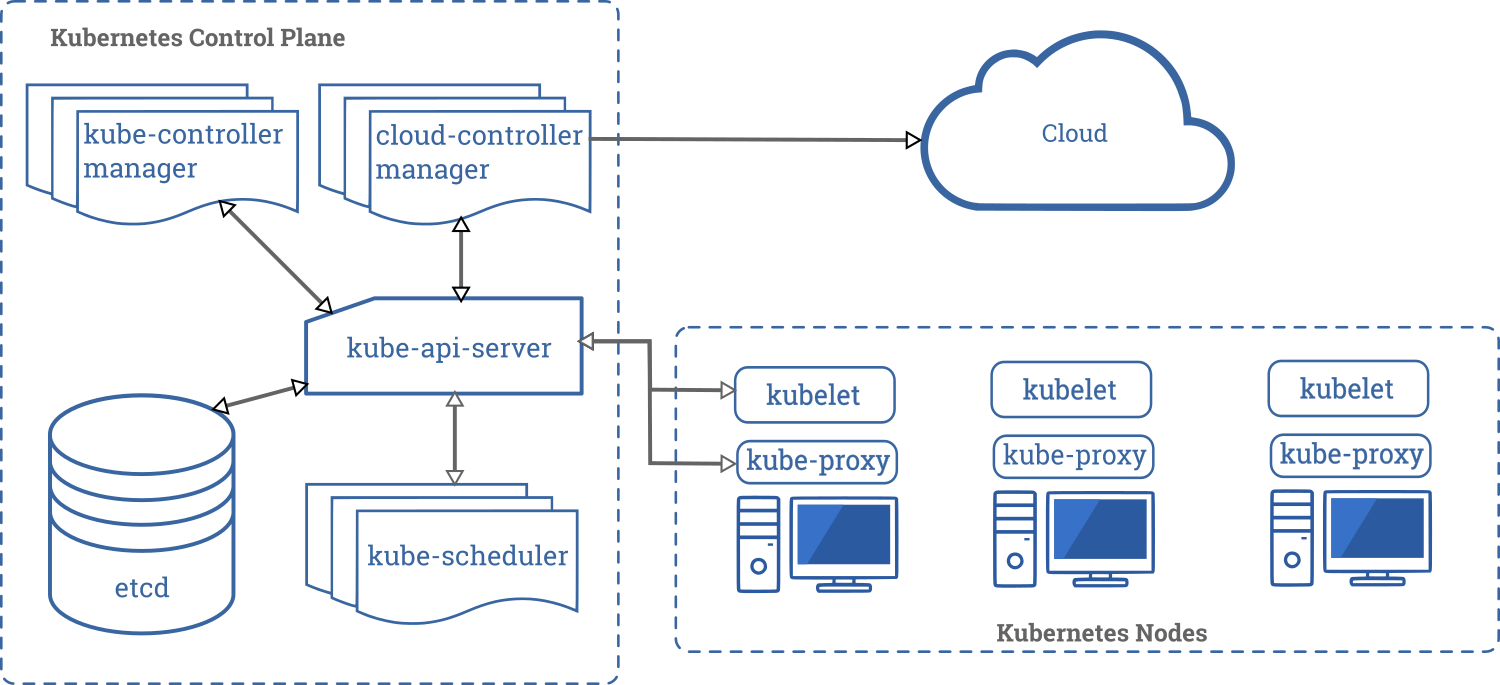
\includegraphics[width=\textwidth]{imgs/components-of-kubernetes.png}
	\captionsource{Components of Kubernetes}{https://kubernetes.io/docs/concepts/overview/components/}
	\label{fig:kube-components}
\end{figure}

\section{Batsim concepts}

\subsection{Limitations}

\section{Translation}

\section{Synchronization}

\chapter{State of the art}

\section{Simulating Kubernetes}

Simulating the Kubernetes ecosystem is a difficult task that hasn't been done
many times. In fact, we have been able to find only two references on the
subject. One is a from an internship, and the other does not have any open
source release.

To our knowledge, there isn't any other project about adapting Simgrid to
Kubernetes.

\subsection{k8s-cluster-simulator}

k8s-cluster-simulator\cite{kubesim} is an internship project written in Go. It
aims at simulating a Kubernetes clusters in order to evaluate schedulers with
basic workloads, with as little changes to schedulers implementation as
possible.

The user can specify resource usage for some pods in a yaml config file (cpu,
memory, gpu) and submit them through an interface. The scheduler is also
submitted through an interface, and that makes the code not exactly plug and
play : the scheduler has to comply with the interface to be evaluated.

This is a simple project useful for understanding some Kubernetes core concepts
and technical details.

\subsection{JoySim simulator from JD.com}

This is a project led by the company JD.com, presented in the \textbf{KubeCon +
	CloudNativeCon North America 2019}\cite{joysim}. It looks like a very
complete, fully fledged Kubernetes cluster simulator, however it is not (yet)
open-source : ``Planning to work with CNCF SIG-Scheduling for an open source
release''.

\section{Kubernetes schedulers}

Gathering knowledge on the scheduling ecosystem in Kubernetes is a first step
in deciding what direction to take with Batkube. It came out that the most
useful resources we could find were the very simple schedulers that were
written as examples or tutorials about writing custom schedulers. These basic
schedulers made the process of writing proof of concepts much easier.


\subsection{Industry grade schedulers}

\subsubsection{Kubernetes scheduler}

kube-scheduler is the de facto scheduler for any Kubernetes
cluster (at least with the native Kubernetes distribution) and can be found in
Kubernetes repository\cite{kube-repo}.

It is a generic scheduler and very effective in most cases.

\subsubsection{kube-batch}

kube-batch\cite{kube-batch} is a batch scheduler developed by the Kubernetes
Scheduling SIG\cite{scheduling-sig}.

It has proven reliable on an industrial size and serves as a base for other scheduling projects (e.g. Volcano\cite{volcano}).

\subsubsection{Poseidon}

\subsection{Example schedulers}

These schedulers helped a great deal in understanding how a scheduler interacts
with the Kubernetes api-server, thanks to their simplicity.

\subsubsection{Bash scheduler}

The bashScheduler\cite{bashScheduler} is a tiny project created demonstrating a
very basic implementation of a random scheduler using only bash, so as to break
down exchanges between the api server and the scheduler with simple http
requests.

It has served as a base upon which the first POC was created.

\subsubsection{Random scheduler}

This project is taken from a tutorial\cite{banzai-tuto} redacted by Banzai
Cloud to guide us through the implementation of a custom scheduler using the go
client\cite{client-go} from kubernetes.
Like the bashScheduler, it randomly binds pods on available nodes. Although, it
takes things to the next level by using the go client thus introducing the
concept of kubernetes informers and using https instead of plain http.

The second POC was built using this scheduler as a base.

\chapter{Implementation}

\section{Batkube architecture}
TODO

\section{Time hijack}
TODO

\subsection{batsky-go}
\SetKwInput{KwInput}{Input}
\SetKwInput{KwOutput}{Output}


\begin{algorithm}[H]
\DontPrintSemicolon
\KwInput{req: request channel, res: result channel map}
\While{Batkube is not ready} {
	wait\;
}
requests = []request\;
\While{req is not empty} {
	m = $<$- req \tcc{Non blocking receive}
	requests = append(requests, m)\;
}
sendToBatkube(requests) \tcc{Only requests with duration > 0 are actually sent. Batkube will always anwser.}
now = responseFromBatkube()\;
\For{m in range requests} {
	res[m.id] $<$-now \tcc{The caller continues execution upon reception}
}

	
\caption{Requester loop}
\label{alg:reqLoop}
\end{algorithm}


\begin{algorithm}[H]
\DontPrintSemicolon
\KwResult{Current simulation time}
\KwInput{d: timer duration, req: request channel, res: response channel map}
\KwOutput{now : simulation time}

\If{requester loop is not running}{
	go runRequesterLoop() \tcc{There can on ly be one loop runing at a time}
}
id = newUUID()\;
m = newRequestMessage(d, id) \tcc{Requests are identified using uuids}
resChannel = newChannel()\;
res[id] = resChannel \tcc{A channel is associated with each request}
req $<$- m \tcc{The code blocks here until request is handled}
now = $<$-resChannel \tcc{The code blocks here until response is sent by the requester loop}
return now\;
\caption{Time request (time.now())}
\label{alg:now}
\end{algorithm}



\chapter{Evaluation}

\chapter{Conclusion}


\printbibliography
\end{document}
